\documentclass[
  shownotes,
  xcolor={svgnames},
  hyperref={colorlinks,citecolor=DarkBlue,linkcolor=andesred,urlcolor=DarkBlue}
  , aspectratio=169]{beamer}
\usepackage{animate}
\usepackage{amsmath}
\usepackage{amsfonts}
\usepackage{amssymb}
\usepackage{pifont}
\usepackage{mathpazo}
%\usepackage{xcolor}
\usepackage{multimedia}
\usepackage{fancybox}
\usepackage[para]{threeparttable}
\usepackage{multirow}
\setcounter{MaxMatrixCols}{30}
\usepackage{subcaption}
\usepackage{graphicx}
\usepackage{lscape}
\usepackage[compatibility=false,font=small]{caption}
\usepackage{booktabs}
\usepackage{ragged2e}
\usepackage{chronosys}
\usepackage{appendixnumberbeamer}
\usepackage{animate}
\setbeamertemplate{caption}[numbered]
\usepackage{color}
%\usepackage{times}
\usepackage{tikz}
\usepackage{comment} %to comment
%% BibTeX settings
\usepackage{natbib}
\bibliographystyle{apalike}
\bibpunct{(}{)}{,}{a}{,}{,}
\setbeamertemplate{bibliography item}{[\theenumiv]}

% Defines columns for bespoke tables
\usepackage{array}
\newcolumntype{L}[1]{>{\raggedright\let\newline\\\arraybackslash\hspace{0pt}}m{#1}}
\newcolumntype{C}[1]{>{\centering\let\newline\\\arraybackslash\hspace{0pt}}m{#1}}
\newcolumntype{R}[1]{>{\raggedleft\let\newline\\\arraybackslash\hspace{0pt}}m{#1}}


\usepackage{xfrac}


\usepackage{multicol}
\setlength{\columnsep}{0.5cm}

% Theme and colors
\usetheme{Boadilla}

% I define a custom pallete
\definecolor{andesred}{HTML}{1B175E}
\definecolor{andesyellow}{HTML}{ffff00}

% Other options
\providecommand{\U}[1]{\protect\rule{.1in}{.1in}}
\usefonttheme{serif}
\setbeamertemplate{itemize items}[default]
\setbeamertemplate{enumerate items}[square]
\setbeamertemplate{section in toc}[circle]


\definecolor{mybackground}{HTML}{1B175E}
\definecolor{myforeground}{HTML}{0000A0}

\setbeamercolor{normal text}{fg=black,bg=white}
\setbeamercolor{alerted text}{fg=andesred}
\setbeamercolor{example text}{fg=black}

\setbeamercolor{background canvas}{fg=myforeground, bg=white}
\setbeamercolor{background}{fg=myforeground, bg=mybackground}
\setbeamercolor{palette tertiary}{fg=myforeground,bg=mybackground}

\setbeamercolor{palette primary}{fg=black, bg=white}
\setbeamercolor{palette secondary}{fg=black, bg=white!10!andesyellow}
\setbeamercolor{palette tertiary}{fg=black, bg=white}


\setbeamercolor{frametitle}{fg=black}
\setbeamercolor{title}{fg=black}
\setbeamercolor{block title}{fg=andesred}
\setbeamercolor{itemize item}{fg=andesred}
\setbeamercolor{itemize subitem}{fg=andesred}
\setbeamercolor{itemize subsubitem}{fg=andesred}
\setbeamercolor{enumerate item}{fg=andesred}
\setbeamercolor{item projected}{bg=gray!30!white,fg=andesred}
\setbeamercolor{enumerate subitem}{fg=andesred}
\setbeamercolor{section number projected}{bg=gray!30!white,fg=andesred}
\setbeamercolor{section in toc}{fg=andesred}
\setbeamercolor{caption name}{fg=andesred}
\setbeamercolor{button}{bg=gray!30!white,fg=andesred}
\setbeamercolor{title in head/foot}{fg=andesred}



\usepackage{fancyvrb}
\newcommand{\VerbBar}{|}
\newcommand{\VERB}{\Verb[commandchars=\\\{\}]}
\DefineVerbatimEnvironment{Highlighting}{Verbatim}{commandchars=\\\{\}}
% Add ',fontsize=\small' for more characters per line
\usepackage{framed}
\definecolor{shadecolor}{RGB}{248,248,248}
\newenvironment{Shaded}{\begin{snugshade}}{\end{snugshade}}
\newcommand{\AlertTok}[1]{\textcolor[rgb]{0.94,0.16,0.16}{#1}}
\newcommand{\AnnotationTok}[1]{\textcolor[rgb]{0.56,0.35,0.01}{\textbf{\textit{#1}}}}
\newcommand{\AttributeTok}[1]{\textcolor[rgb]{0.77,0.63,0.00}{#1}}
\newcommand{\BaseNTok}[1]{\textcolor[rgb]{0.00,0.00,0.81}{#1}}
\newcommand{\BuiltInTok}[1]{#1}
\newcommand{\CharTok}[1]{\textcolor[rgb]{0.31,0.60,0.02}{#1}}
\newcommand{\CommentTok}[1]{\textcolor[rgb]{0.56,0.35,0.01}{\textit{#1}}}
\newcommand{\CommentVarTok}[1]{\textcolor[rgb]{0.56,0.35,0.01}{\textbf{\textit{#1}}}}
\newcommand{\ConstantTok}[1]{\textcolor[rgb]{0.00,0.00,0.00}{#1}}
\newcommand{\ControlFlowTok}[1]{\textcolor[rgb]{0.13,0.29,0.53}{\textbf{#1}}}
\newcommand{\DataTypeTok}[1]{\textcolor[rgb]{0.13,0.29,0.53}{#1}}
\newcommand{\DecValTok}[1]{\textcolor[rgb]{0.00,0.00,0.81}{#1}}
\newcommand{\DocumentationTok}[1]{\textcolor[rgb]{0.56,0.35,0.01}{\textbf{\textit{#1}}}}
\newcommand{\ErrorTok}[1]{\textcolor[rgb]{0.64,0.00,0.00}{\textbf{#1}}}
\newcommand{\ExtensionTok}[1]{#1}
\newcommand{\FloatTok}[1]{\textcolor[rgb]{0.00,0.00,0.81}{#1}}
\newcommand{\FunctionTok}[1]{\textcolor[rgb]{0.00,0.00,0.00}{#1}}
\newcommand{\ImportTok}[1]{#1}
\newcommand{\InformationTok}[1]{\textcolor[rgb]{0.56,0.35,0.01}{\textbf{\textit{#1}}}}
\newcommand{\KeywordTok}[1]{\textcolor[rgb]{0.13,0.29,0.53}{\textbf{#1}}}
\newcommand{\NormalTok}[1]{#1}
\newcommand{\OperatorTok}[1]{\textcolor[rgb]{0.81,0.36,0.00}{\textbf{#1}}}
\newcommand{\OtherTok}[1]{\textcolor[rgb]{0.56,0.35,0.01}{#1}}
\newcommand{\PreprocessorTok}[1]{\textcolor[rgb]{0.56,0.35,0.01}{\textit{#1}}}
\newcommand{\RegionMarkerTok}[1]{#1}
\newcommand{\SpecialCharTok}[1]{\textcolor[rgb]{0.00,0.00,0.00}{#1}}
\newcommand{\SpecialStringTok}[1]{\textcolor[rgb]{0.31,0.60,0.02}{#1}}
\newcommand{\StringTok}[1]{\textcolor[rgb]{0.31,0.60,0.02}{#1}}
\newcommand{\VariableTok}[1]{\textcolor[rgb]{0.00,0.00,0.00}{#1}}
\newcommand{\VerbatimStringTok}[1]{\textcolor[rgb]{0.31,0.60,0.02}{#1}}
\newcommand{\WarningTok}[1]{\textcolor[rgb]{0.56,0.35,0.01}{\textbf{\textit{#1}}}}
\usepackage{graphicx}
\makeatletter

\makeatother






%%%%%%%%%%%%%%% BEGINS DOCUMENT %%%%%%%%%%%%%%%%%%

\AtBeginSection[]
{
    \begin{frame}
        \frametitle{Agenda}
        \tableofcontents[currentsection]
    \end{frame}
}

\begin{document}

\title{Linear Regression and Resampling Methods for Uncertainty}
\subtitle{Big Data y Machine Learning para Economía Aplicada}
\date{}

\author[Sarmiento-Barbieri]{Ignacio Sarmiento-Barbieri}
\institute[Uniandes]{Universidad de los Andes}


\begin{frame}[noframenumbering]
\maketitle
\end{frame}


\begin{frame}
\frametitle{Agenda}

\tableofcontents


\end{frame}
%----------------------------------------------------------------------%
\section{Review}
%----------------------------------------------------------------------%
\begin{frame}
\frametitle{Predicting Well}


\begin{align}
y=f(X)+u
\end{align}

\begin{itemize}
  \item Interest on predicting $y$
  \medskip
  \item Model? We  treat $f()$ as a black box, and any approximation $\hat{f}()$ that yields a good prediction is good enough ({\it ``Whatever works, works...''}).
  \medskip
  \item How do we measure ``what works''?
  
  \medskip
  \begin{align}
E(y-\hat y)^2 &= E(f(X)+u - \hat f(X))^2 
\end{align}

\end{itemize}
\end{frame}
%----------------------------------------------------------------------%
\begin{frame}
\frametitle{Predicting Well}

\begin{align}
E(y-\hat y)^2  &= \underset{Reducible}{\underbrace{[f(X)-\hat{f}(X)]^{2}}}+\underset{Irreducible}{\underbrace{Var(u)}}
\end{align}
\begin{align}
  MSE = Bias^2 (\hat f(X))+V (\hat f(X)) +\underset{Irreducible}{\underbrace{Var(u)}}
\end{align}
\end{frame}

%----------------------------------------------------------------------%
\begin{frame}
\frametitle{The Bias-Variance Trade-Off}
\begin{figure}[H] \centering
  \centering
  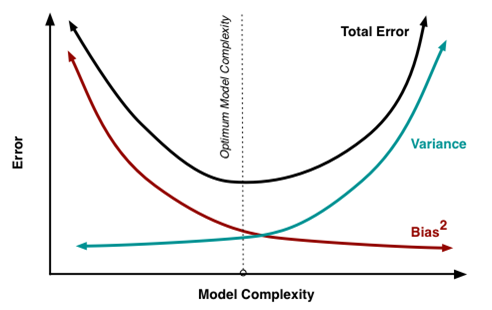
\includegraphics[scale=0.35]{figures/medium_bias_variance_trade_off.png}
  \\
  \tiny
  Source: https://tinyurl.com/y4lvjxpc
\end{figure}
\begin{itemize}
  
  \item The best kept secret: tolerating some bias is possible to reduce V($\hat f(X)$) and lower MSE
  
\end{itemize}

\end{frame}

%----------------------------------------------------------------------%
\begin{frame}
\frametitle{Linear Regression}

\begin{align}
y&=f(X)+u \\
  & = \beta_0 + \beta_1 X_1 + \dots + \beta_p X_p  + u \\
  &= X\beta + u
\end{align}


\begin{itemize}
\item  If $f(X)=X\beta$, obtaining $f(.)$ boils down to obtaining $\beta$

 \medskip
\item where  we can obtain $\beta$ minimizing RSS (SSR)
 \medskip
\begin{align}
\hat \beta=(X'X)^{-1}X'y
\end{align}

 \medskip
\item Involves inverting a $k\times k$ matrix $X'X$
 \medskip
\item requires allocating $O (nk+k^2)$ if n is "big" we cannot store this in memory

\end{itemize} 

\end{frame}

%----------------------------------------------------------------------%
\begin{frame}
\frametitle{Linear Regression}


\begin{itemize}
\item Gauss-Markov Theorem
 \medskip
\begin{itemize}
\item If it is assumed that $E(u|X) = 0$ and $E(uu'|X) = \sigma^2I$ in the linear regression model $y = X\beta+u $, then the OLS estimator $\hat{\beta}$ is more efficient than any other linear unbiased estimator $\tilde{\beta}$, in the sense that $Var(\tilde{\beta})-Var(\hat{\beta}$ is a positive semidefinite matrix. 

\end{itemize}
 \medskip
 \item An informal way of stating this theorem is to say that $\hat{\beta}$ is the best linear unbiased estimator, or BLUE for short.
 \medskip
 \item In other words, the OLS estimator is more efficient than any other linear unbiased estimator.

\end{itemize}

\end{frame}

%----------------------------------------------------------------------%
\begin{frame}
\frametitle{Linear Regression}

\begin{itemize}

\item Let's consider the simple case with two regressors:

\begin{align}
y_{i}=\beta_{0}+\beta_{1}x_{1i}+\beta_{2}x_{2i}+u
\end{align}


\item with $E(u)=0$, $cov(x_{1},u)=0$, $cov(x_{2},u)=0$ and $E(u^2|x_1,x_2) = \sigma^2$
\medskip
\item OLS says we should choose the estimators $\hat{\beta}_{0}$,$\hat{\beta}_{1}$, $\hat{\beta}_{2}$ of $\beta_{0}$, $\beta_{1}$, $\beta_{2} $ such that we minimize the Sum of Square Residual (SSR) or the Residual Sum of Squares (RSS)

\begin{align}
\mathcal{L}&= \sum\left(y_{i}-\hat{y}_i\right)^{2} \\
&=\sum\left(y_{i}-\hat{\beta}_{0}-\hat{\beta}_{1}x_{1i}-\hat{\beta}_{2}x_{2i}\right)^{2} 
\end{align}

\end{itemize}
\end{frame}


%----------------------------------------------------------------------%
\begin{frame}
\frametitle{Linear Regression}

\begin{itemize}

\item The solution then comes from solving the FOC (and checking the SOC)

\begin{align}
\frac{\partial\mathcal{L}}{\partial\hat{\beta}_{0}}&=\sum2\left(y_{i}-\hat{\beta}_{0}-\hat{\beta}_{1}x_{1i}-\hat{\beta}_{2}x_{2i}\right)(-1)=0 \\
\frac{\partial\mathcal{L}}{\partial\hat{\beta}_{1}}&=\sum2\left(y_{i}-\hat{\beta}_{0}-\hat{\beta}_{1}x_{1i}-\hat{\beta}_{2}x_{2i}\right)(-x_{1i})=0 \\
\frac{\partial\mathcal{L}}{\partial\hat{\beta}_{2}}&=\sum2\left(y_{i}-\hat{\beta}_{0}-\hat{\beta}_{1}x_{1i}-\hat{\beta}_{2}x_{2i}\right)(-x_{2i})=0
\end{align}

\item Solving, for example, for $\hat{\beta}_2$ we have
\begin{align}
\hat{\beta}_{2}=\frac{\sum(x_{1i}-\bar{x}_{1})^{2}\sum(x_{2i}-\bar{x}_{2})y_{i}-\left( \sum x_{1i}x_{2i}-n\bar{x}_{1}\bar{x}_{2} \right)\sum(x_{1i}-\bar{x}_{1})y_{i}}{\sum(x_{1i}-\bar{x}_{1})^{2}\sum(x_{2i}-\bar{x}_{2})^{2}-\left( \sum x_{1i}x_{2i}-n\bar{x}_{1}\bar{x}_{2}\right)^{2}}
\end{align}

\end{itemize}
\end{frame}



%----------------------------------------------------------------------%
\begin{frame}
\frametitle{Goodness-of-fit. In  sample performance}

\begin{itemize}
\item The mechanics of OLS lead to a very simple measure of \emph{goodness of fit}, the $R^2$, or \emph{coefficient of determination}, one of the most used and abused in the practice of econometrics and statistics. 
\medskip
\item The starting point is the following \emph{sum of squares decomposition}:
\medskip
\[ \sum \tilde{y}_i^2  = \sum \hat \tilde{y}_i^2 + \sum e_i^2,\] 

\item where $\tilde{y}_i \equiv Y_i - \bar Y$, $\hat y_i \equiv \hat Y_i - \bar Y$ and $e_i$ are OLS residuals. The decomposition holds for any number of explanatory variables.
\medskip

\item where $\tilde{y}_i \equiv y_i - \bar y$, $\hat \tilde{y}_i \equiv \hat \tilde{y}_i - \bar y$ and $e_i$ are OLS residuals. 
\medskip
\item The decomposition holds for any number of explanatory variables,  the derivation uses the FOC above
\end{itemize}
\end{frame}
%----------------------------------------------------------------------%
\begin{frame}
\frametitle{Goodness-of-fit. In  sample performance}

\begin{itemize}
  \item To get some intuition, divide by $n$ in both sides of the decomposition $\rightarrow$ Each term resembles sort of a variance.
  \item  The decomposition suggests that the total variability of $Y$ can be `explained' by the variability in the fitted model (ESS) plus that of the error term (RSS). 
  $$ 
  TSS = ESS + RSS 
  $$

\item The \emph{coefficient of determination}, or $R^2$ for a given regression model is defined as 

\[ R^2 \equiv \frac{ESS}{TSS}\]
\item which we can also rewrite as 
\[ R^2 \equiv 1 - \frac{RSS}{TSS}\]

\end{itemize}

% Here is a list of properties of $R^2$

% \begin{enumerate}
%     \item $0 \leq R^2 \leq 1$. First, $R^2$ is by definition the ratio of two positive numbers (ESS and TSS), so it cannot be negative. Second, from the decomposition, $ESS \leq TSS$ hence $ESS/TSS \leq 1$.
%     \item $R^2=1$ if and only if $e_i=0$ for all observations. This comes from $R^2 =0$ iff SSR=0, which in turn requires that all $e_i$'s are zero. This in turn implies that $Y_i = \hat Y_i$. That is, when $R^2=1$, the model fits the data perfectly.
%     \item $R^2=0$ if and only if all slope coefficients are zero. In such case, the best model is the `just intercept model' of chapter 1, which implies that $\hat Y_i = \bar Y$, which leads to ESS=0 and $R^2=0$. That is, $R^2=0$ when none of the explanatory variables help represent $Y$ beyond an intercept, estimated by the $\bar Y$.
%     \item $\hat \beta$ maximizes $R^2$. Note that TSS does not depend on the fitted model. Then, from $R^2 = 1-RSS/TSS$, if $\hat \beta$ minimizes RSS, then it has to maximize $R^2$ since TSS is unaffected by this minimization. Consequently, maximizing $R^2$ and minimizing $RSS$ are not contradicting goals,they lead exactly to the same solution. 
%     \item $R_2$ is non decreasing in the number of explanatory variables. This a crucial property that is also tricky to think. Suppose that there are two models. Model 1 includes $K_1$ variables. Model 2 is a larger version, that includes more variables, say $K_2$, with $K_2 > K_1$. It is important to remark that model 2 is not just `larger' but that explanatory variables in model 1 are actually a subset of those in model 2. Denote with $RSS_2$ the residual sum of squares in model 2, and $RSS_1$ that of model 1. Model 1 can be thought as a restricted version of model 2. That is, en each case RSS results from finding OLS coefficients to minimize it. But whereas in model 2, the minimization proceeds `freely', in model 1 it is as it can pick any value for the coefficients, but it has to set zeros at the values of variables not in modelo 1. That is, excluding variables is equivalent to setting their coefficients equal to zero. Consequently, $RSS_2$ is a free minimun and $RSS_1$ a restricted one, and hence $RSS_2 \leq RSS_2$. Replacing in the definition of $R^2$ we get the result. 
%     \item When $n=K$, $R^2=1$. This is scary: when you add as many regressors as observations, the model fits the data perfectly \emph{no matter what the explanatory variables are}. A proof requires some matrix manipulations, we will do it in the Appendix. 
% \end{enumerate}

% The key point is that $R^2$ is a measure of \emph{in sample} performance. Regarding complexity, property 5 implies that the criterion of maximizing $R^2$ favors large models. Out of sample prediction? Then link with the next chapter on overfit and out of sample prediction. 

% \end{itemize}

\end{frame}
%----------------------------------------------------------------------%
\begin{frame}[t]
\frametitle{Goodness-of-fit. In  sample performance}
\begin{itemize}
  \item $R_2$ is non decreasing in the number of explanatory variables

\end{itemize}
\end{frame}
%----------------------------------------------------------------------%
\begin{frame}
\frametitle{ High Leverage Points}

\begin{itemize}
  \item  Outliers are observations for which the response $y_i$ is unusual given the predictor $x_i$.
  \medskip
  \item In contrast, observations with high leverage high have an unusual value for $x_i$.

  \begin{figure}[H] \centering
    \centering
    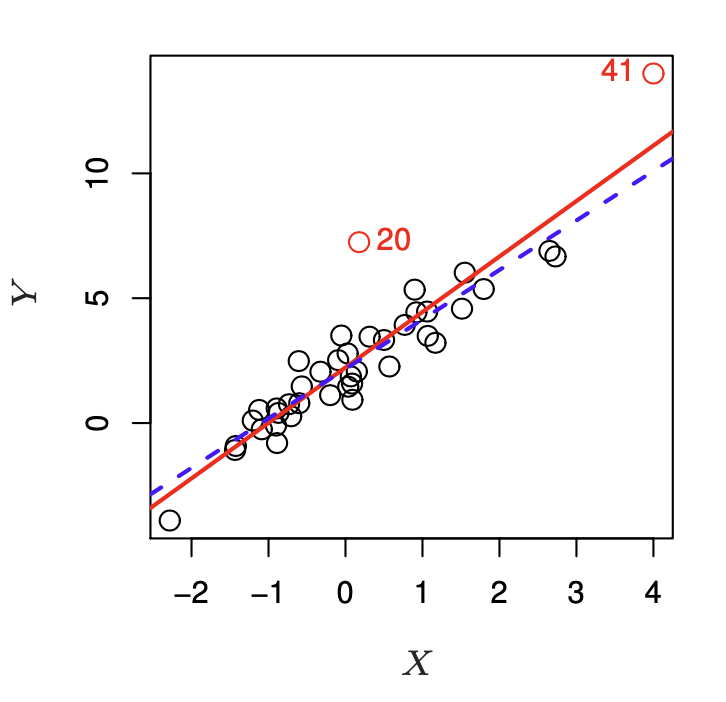
\includegraphics[scale=0.45]{figures/leverage.png}
  \end{figure}

\end{itemize}

\end{frame}
%----------------------------------------------------------------------%
\begin{frame}
\frametitle{ High Leverage Points}

\begin{itemize}
  \item Suppose the simple model 
  $$
 y =  \beta_0 + \beta_1 x + u
  $$

  \item the solution for $\hat{\beta}_1$ is

  \begin{align}
  \hat{\beta}_1 = \frac{\sum(x_{i}-\bar{x})y_{i}}{  \sum(x_{i}-\bar{x})^{2}}= \sum c_i y_i
  \end{align}
  \item the solution for $\hat{\beta}_0$ is
  \begin{align}
  \hat{\beta}_0 = \bar{y}-\hat{\beta}_1 \bar{x} =\frac{1}{n}\sum y_i - \bar{x}\sum c_i y_i
  \end{align}
  \item With a bit of algebra we can write
  \begin{align}
  \hat{y}_i = \sum \left( \frac{1}{n} +\frac{(x_i-\bar{x})^2 }{\sum(x_{i}-\bar{x})^{2}} \right) y_i
  \end{align}
  \begin{align}
  \hat{y}_i = \sum h_i y_i
  \end{align}

\end{itemize}


\end{frame}
%----------------------------------------------------------------------%
\section{Uncertainty: Motivation}
%----------------------------------------------------------------------%

%----------------------------------------------------------------------%
\begin{frame}
\frametitle{Motivation}

\begin{itemize}
  \item The real world is messy. 
  \medskip
  \item Recognizing this mess will differentiate a sophisticated and useful analysis from one that is hopelessly naive. 
  \medskip
  \item This is especially true for highly complicated models, where it becomes tempting to confuse signal with noise and hence “overfit.” 
  \medskip
  \item The ability to deal with this mess and noise is the most important skill you need.
\end{itemize}
\end{frame}

%----------------------------------------------------------------------%
\begin{frame}
\frametitle{ Uncertainty in Linear Regression}

\begin{itemize}
  \item To get a measure of the uncertainty, precision or variability of our estimates we need a measure
  \medskip
  \item We can estimate the Variance of our estimators
  \medskip
  \item For example for
  \begin{align}
  y_{i}=\beta_{0}+\beta_{1}x_{1i}+u
  \end{align}
  \begin{align}
  \hat{\beta}_{1} = \frac{\sum(x_{1i}-\bar{x}_{1})y_{i}}{\sum(x_{1i}-\bar{x}_{1})^{2}}
  \end{align}
  \begin{align}
  Var(\hat{\beta}_{1}) = \frac{\sigma^2}{\sum(x_{1i}-\bar{x}_{1})^{2}}=\frac{\sigma^2}{nVar(x_{1i})}
  \end{align}
\end{itemize}

\end{frame}

%----------------------------------------------------------------------%
\begin{frame}
\frametitle{ Uncertainty in Linear Regression}

\begin{itemize}
  \item Let's go back to our two variable model
  \medskip
  \begin{align}
    y_{i}=\beta_{0}+\beta_{1}x_{1i}+\beta_{2}x_{2i}+u
  \end{align}
  \item the solution for $\beta_2$ was:
  \medskip
  \begin{align}
\hat{\beta}_{2}=\frac{\sum(x_{1i}-\bar{x}_{1})^{2}\sum(x_{2i}-\bar{x}_{2})y_{i}-\left( \sum x_{1i}x_{2i}-n\bar{x}_{1}\bar{x}_{2} \right)\sum(x_{1i}-\bar{x}_{1})y_{i}}{\sum(x_{1i}-\bar{x}_{1})^{2}\sum(x_{2i}-\bar{x}_{2})^{2}-\left( \sum x_{1i}x_{2i}-n\bar{x}_{1}\bar{x}_{2}\right)^{2}}
\end{align}
\end{itemize}
\end{frame}

%----------------------------------------------------------------------%
\begin{frame}
\frametitle{ Uncertainty in Linear Regression}
\begin{itemize}
  \item The variance?
  \medskip
  \begin{align}
    Var(\hat{\beta}_{2})=\frac{\sigma^2}{n Var(x_2)(1-R^2_2)}
  \end{align}
   \medskip
   \item this is a special case of the very general formula
  \begin{align}
    Var(\hat{\beta}_{k})=\frac{\sigma^2}{n Var(x_k)(1-R^2_k)}
  \end{align}
  
\end{itemize}
\end{frame}
%----------------------------------------------------------------------%
\section{What are resampling methods?}
%----------------------------------------------------------------------%
\begin{frame}[fragile]
\frametitle{What are resampling methods?}

\begin{itemize}
\item Tools that involves repeatedly drawing samples from a training set and refitting a model of interest on each sample in order to obtain more information about the fitted model
\medskip
\begin{itemize}
  \item Parameter Assessment: estimate standard errors
  \medskip
  \item Model Assessment: estimate test error rates 
  \medskip
  \item Model Selection: select the appropriate level of model flexibility
  \medskip
  \item They are computationally expensive! But these days we have powerful computers
\end{itemize}
\end{itemize}

\end{frame}

%----------------------------------------------------------------------%
%----------------------------------------------------------------------%
\section{The Bootstrap}
%----------------------------------------------------------------------%
%----------------------------------------------------------------------%
\begin{frame}[fragile]
\frametitle{The Bootstrap}
\framesubtitle{Introduction}

\begin{itemize}
  \item Suppose we have $y_1,y_2,\dots,y_n$ iid $Y\sim(\mu,\sigma^2)$ (both finite)
  \medskip
  \item We want to estimate 
  \begin{align}
    Var(\bar{Y})
  \end{align}

\end{itemize}


 \end{frame}
%----------------------------------------------------------------------%
\begin{frame}[fragile]
\frametitle{The Bootstrap}
\framesubtitle{Introduction}
\begin{itemize}
  \item Alternative way (no formula!)
  \medskip
  \begin{enumerate}
    \item From the $n$ original data points $y_1,y_2,\dots,y_n$ take a sample {\it with replacement} of size $n$
    \medskip
    \item Calculate the sample average of this {\it ``pseudo-sample''}
    \medskip
    \item Repeat this B times.
    \medskip
    \item Compute the variance of the B means
  
  \end{enumerate}

\end{itemize}

 
 \end{frame}
%----------------------------------------------------------------------%
\begin{frame}[fragile]
\frametitle{The Bootstrap}
\framesubtitle{Introduction}

\begin{itemize}
  \item The bootstrap is a widely applicable and extremely powerful statistical tool that can be used to quantify the uncertainty associated with a given estimator or statistical learning method. 
  \medskip
  \item In German the expression {\it an den eigenen Haaren aus dem Sumpf zu ziehen} nicely captures the idea of the bootstrap – {\it ``to pull yourself out of the swamp  by your own hair.''} 

\medskip

\begin{figure}
  
\includegraphics[scale=.3]{figures/pelos.jpg}
\end{figure}
\end{itemize}

 \end{frame}
%----------------------------------------------------------------------%
\begin{frame}[fragile]
\frametitle{The Bootstrap}
\framesubtitle{Introduction}
\begin{itemize}
\item {\bf Key Innovation}: The sample itself is used to assess the precision of the estimate. 
  \medskip
  \item Why would this work? 
  \medskip
  \item Remember that uncertainty arises from the randomness inherent to our data-generating process 
  \medskip
  \item So if we can approximately simulate this randomness, then we can approximately quantify our uncertainty.
  
\end{itemize}



 \end{frame}
%----------------------------------------------------------------------%
\begin{frame}[fragile]
\frametitle{The Bootstrap}
\framesubtitle{Introduction}

\begin{itemize}

  \item There are two key properties of bootstrapping that make this seemingly crazy idea actually work. 
  \medskip
  \begin{enumerate}
  \item Each bootstrap sample must be of the same size (N) as the original sample
  \medskip
  \item Each bootstrap sample must be taken with replacement from the original sample
\end{enumerate}

\end{itemize}
 \end{frame}
%----------------------------------------------------------------------%
\begin{frame}[fragile]
\frametitle{Sampling with replacement}


\begin{figure}
  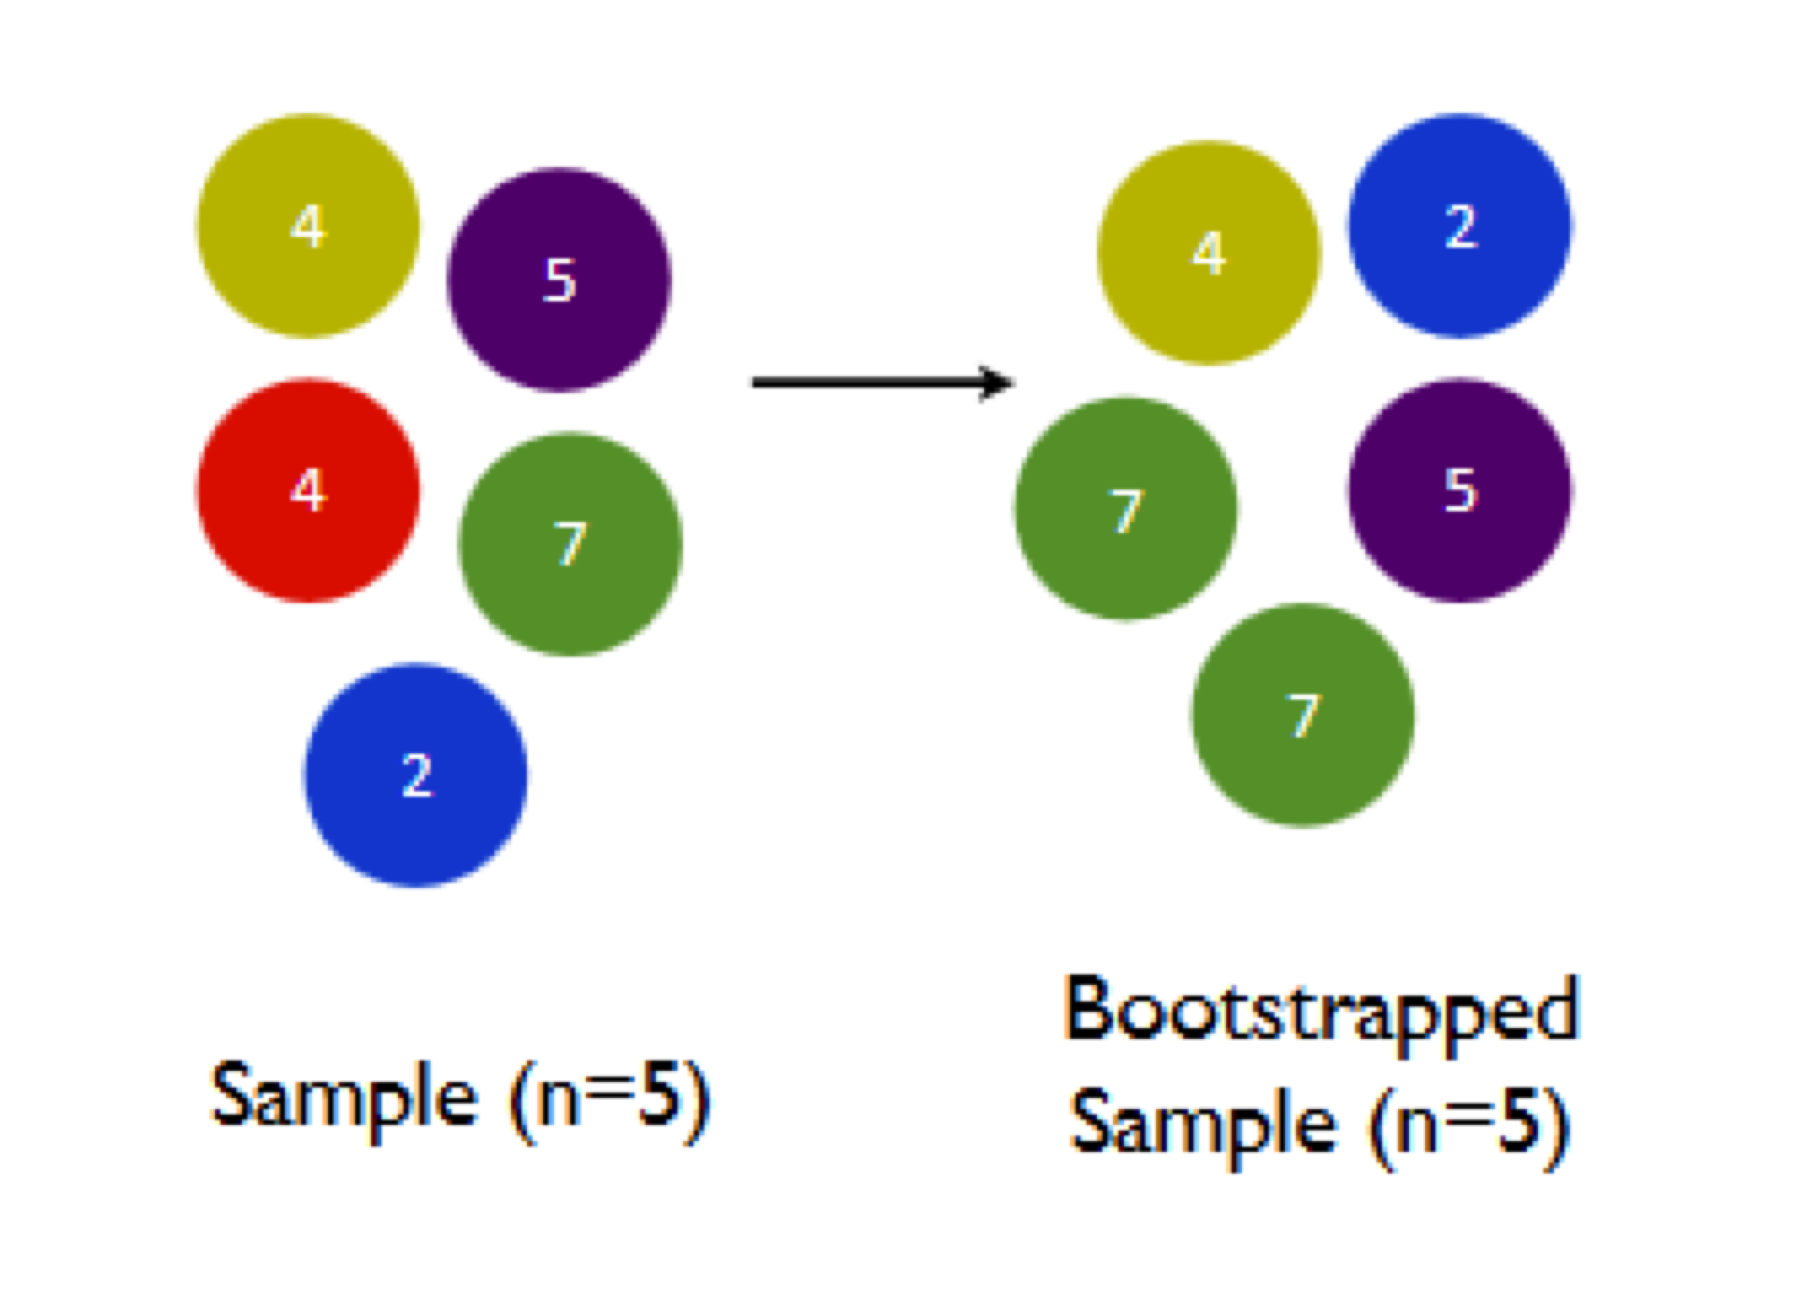
\includegraphics[scale=.3]{figures/bootstrap_cartoon1.png}
\end{figure}

\end{frame}
%----------------------------------------------------------------------%
\begin{frame}[fragile]
\frametitle{Sampling with replacement}
\framesubtitle{Resampling creates synthetic variability}
\begin{figure}
  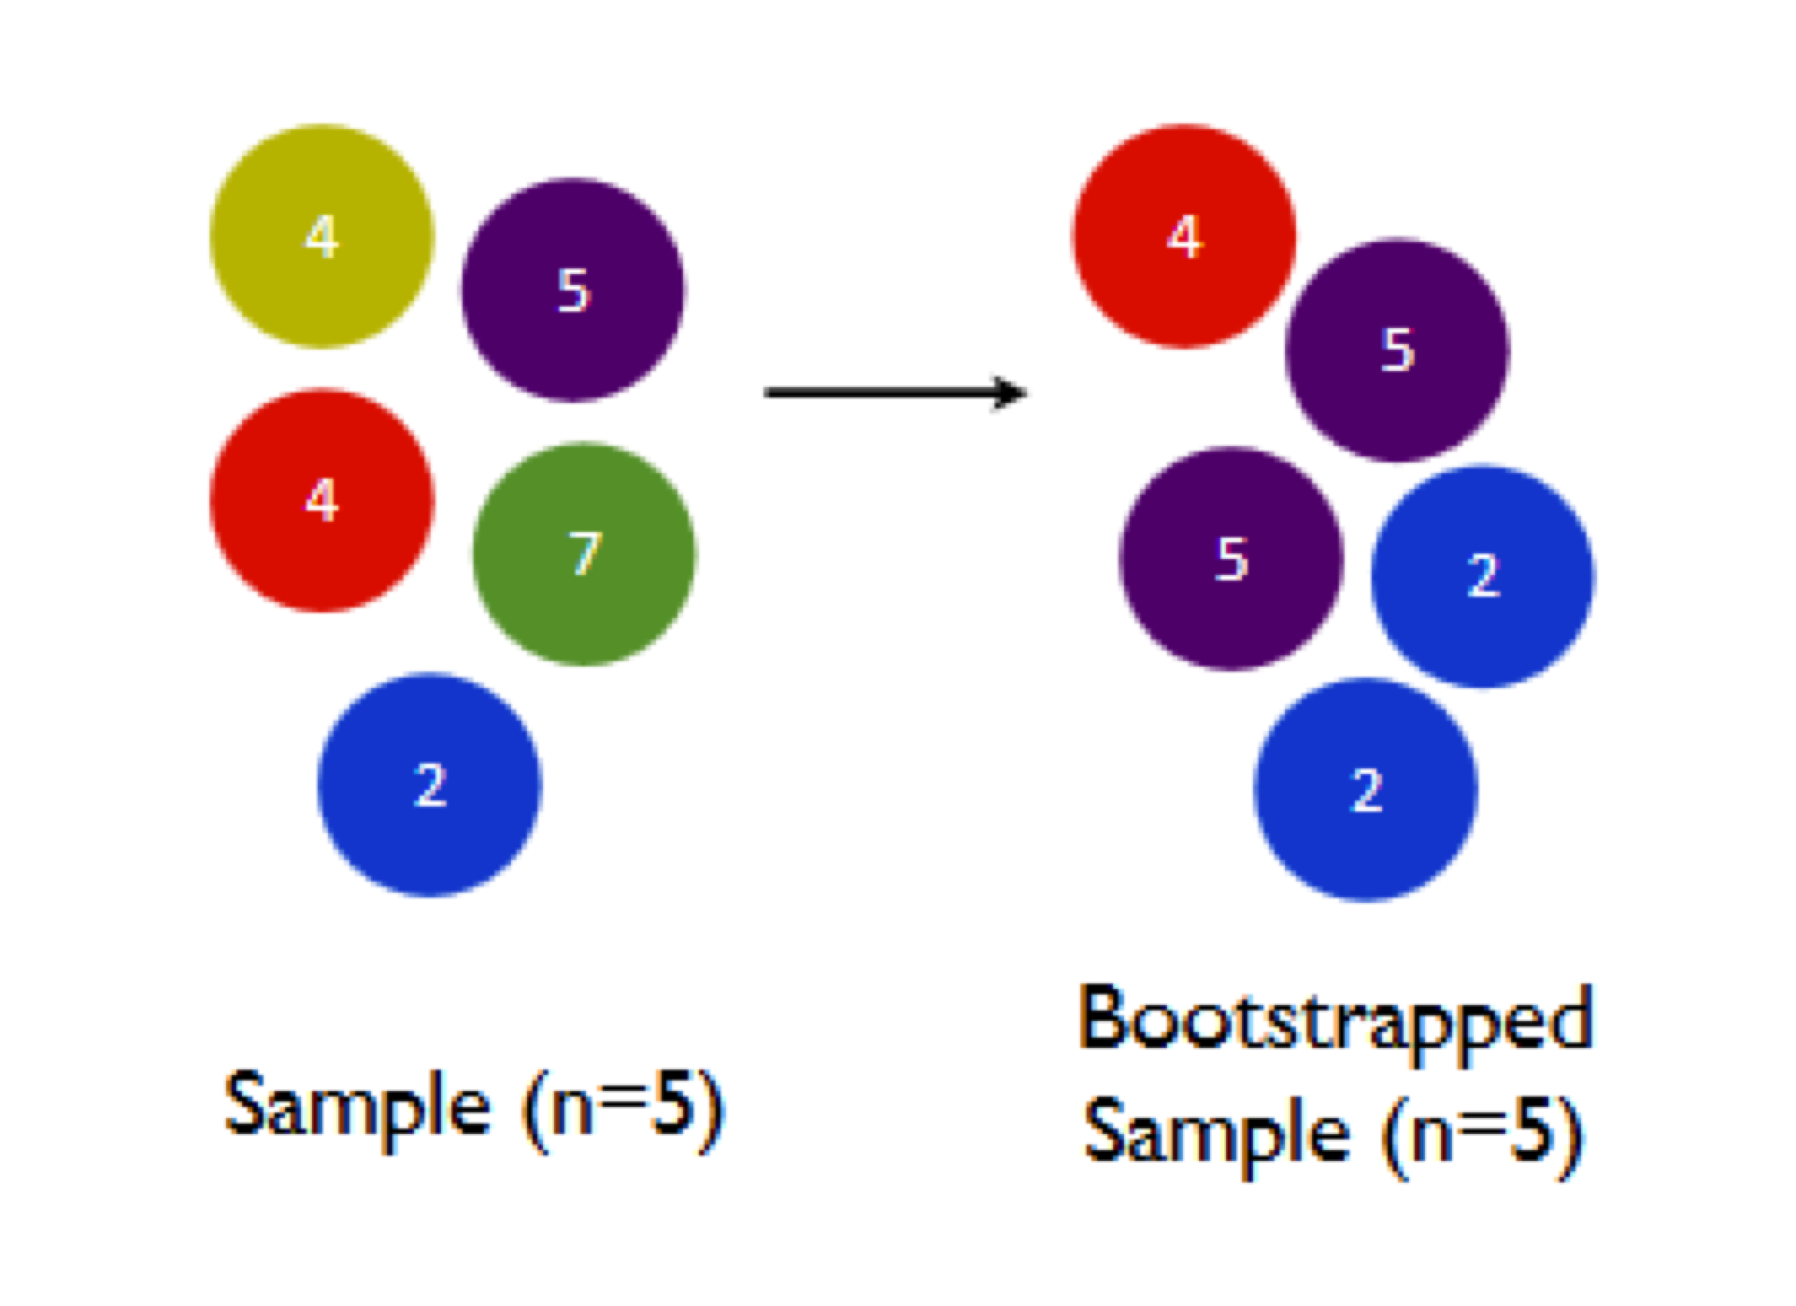
\includegraphics[scale=.3]{figures/bootstrap_cartoon2.png}
\end{figure}

\end{frame}
%----------------------------------------------------------------------%
\begin{frame}[fragile]
\frametitle{Sampling with replacement}
\framesubtitle{Resampling creates synthetic variability}

\begin{figure}
  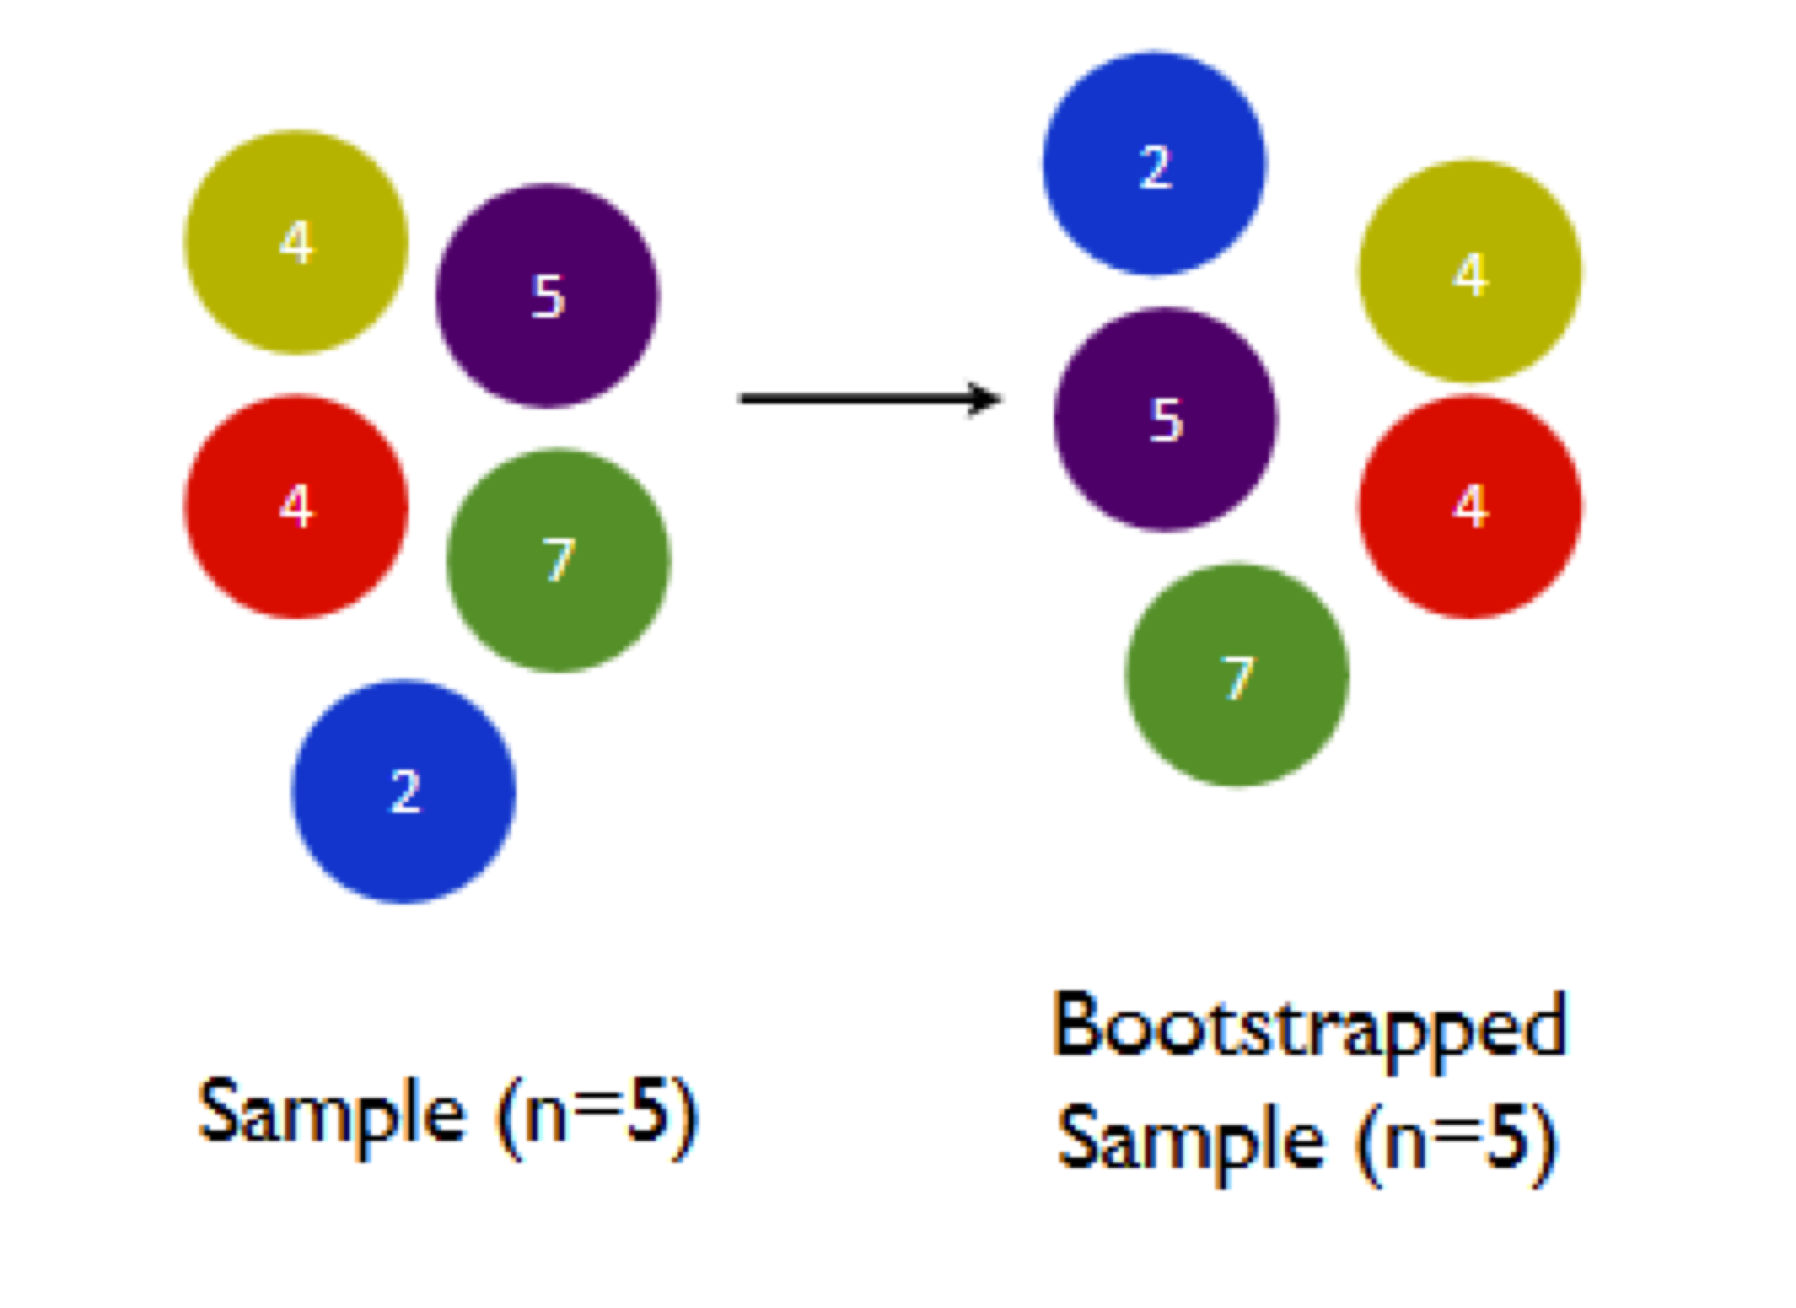
\includegraphics[scale=.3]{figures/bootstrap_cartoon3.png}
\end{figure}

\end{frame}
%----------------------------------------------------------------------%
\begin{frame}[fragile]
\frametitle{The Bootstrap}


\begin{itemize}
  \item In general terms:
    \begin{itemize}
      \item $Y_i$ $i=1,\dots,n$
      \item $\theta$ is the magnitude of interest
    \end{itemize}
    \item To calculate it's variance
   \begin{enumerate}
    \item Sample of size $n$ with replacement ({\it bootstrap sample})
    \medskip
    \item Compute $\hat{\theta}_j$ $j=1,\dots,B$
    \medskip
    \item Repeat $B$ times
    \medskip
    \item Calculate
    \begin{align}
    \hat{V}(\hat{\theta})_B =\frac{1}{B}\sum_{j=1}^B (\hat{\theta}_j- \bar{\hat{\theta}})^2
    \end{align}
   \end{enumerate}
  \medskip


\end{itemize}
 
 \end{frame}
%----------------------------------------------------------------------%
\begin{frame}[fragile]
\frametitle{The Bootstrap}


\begin{figure}
  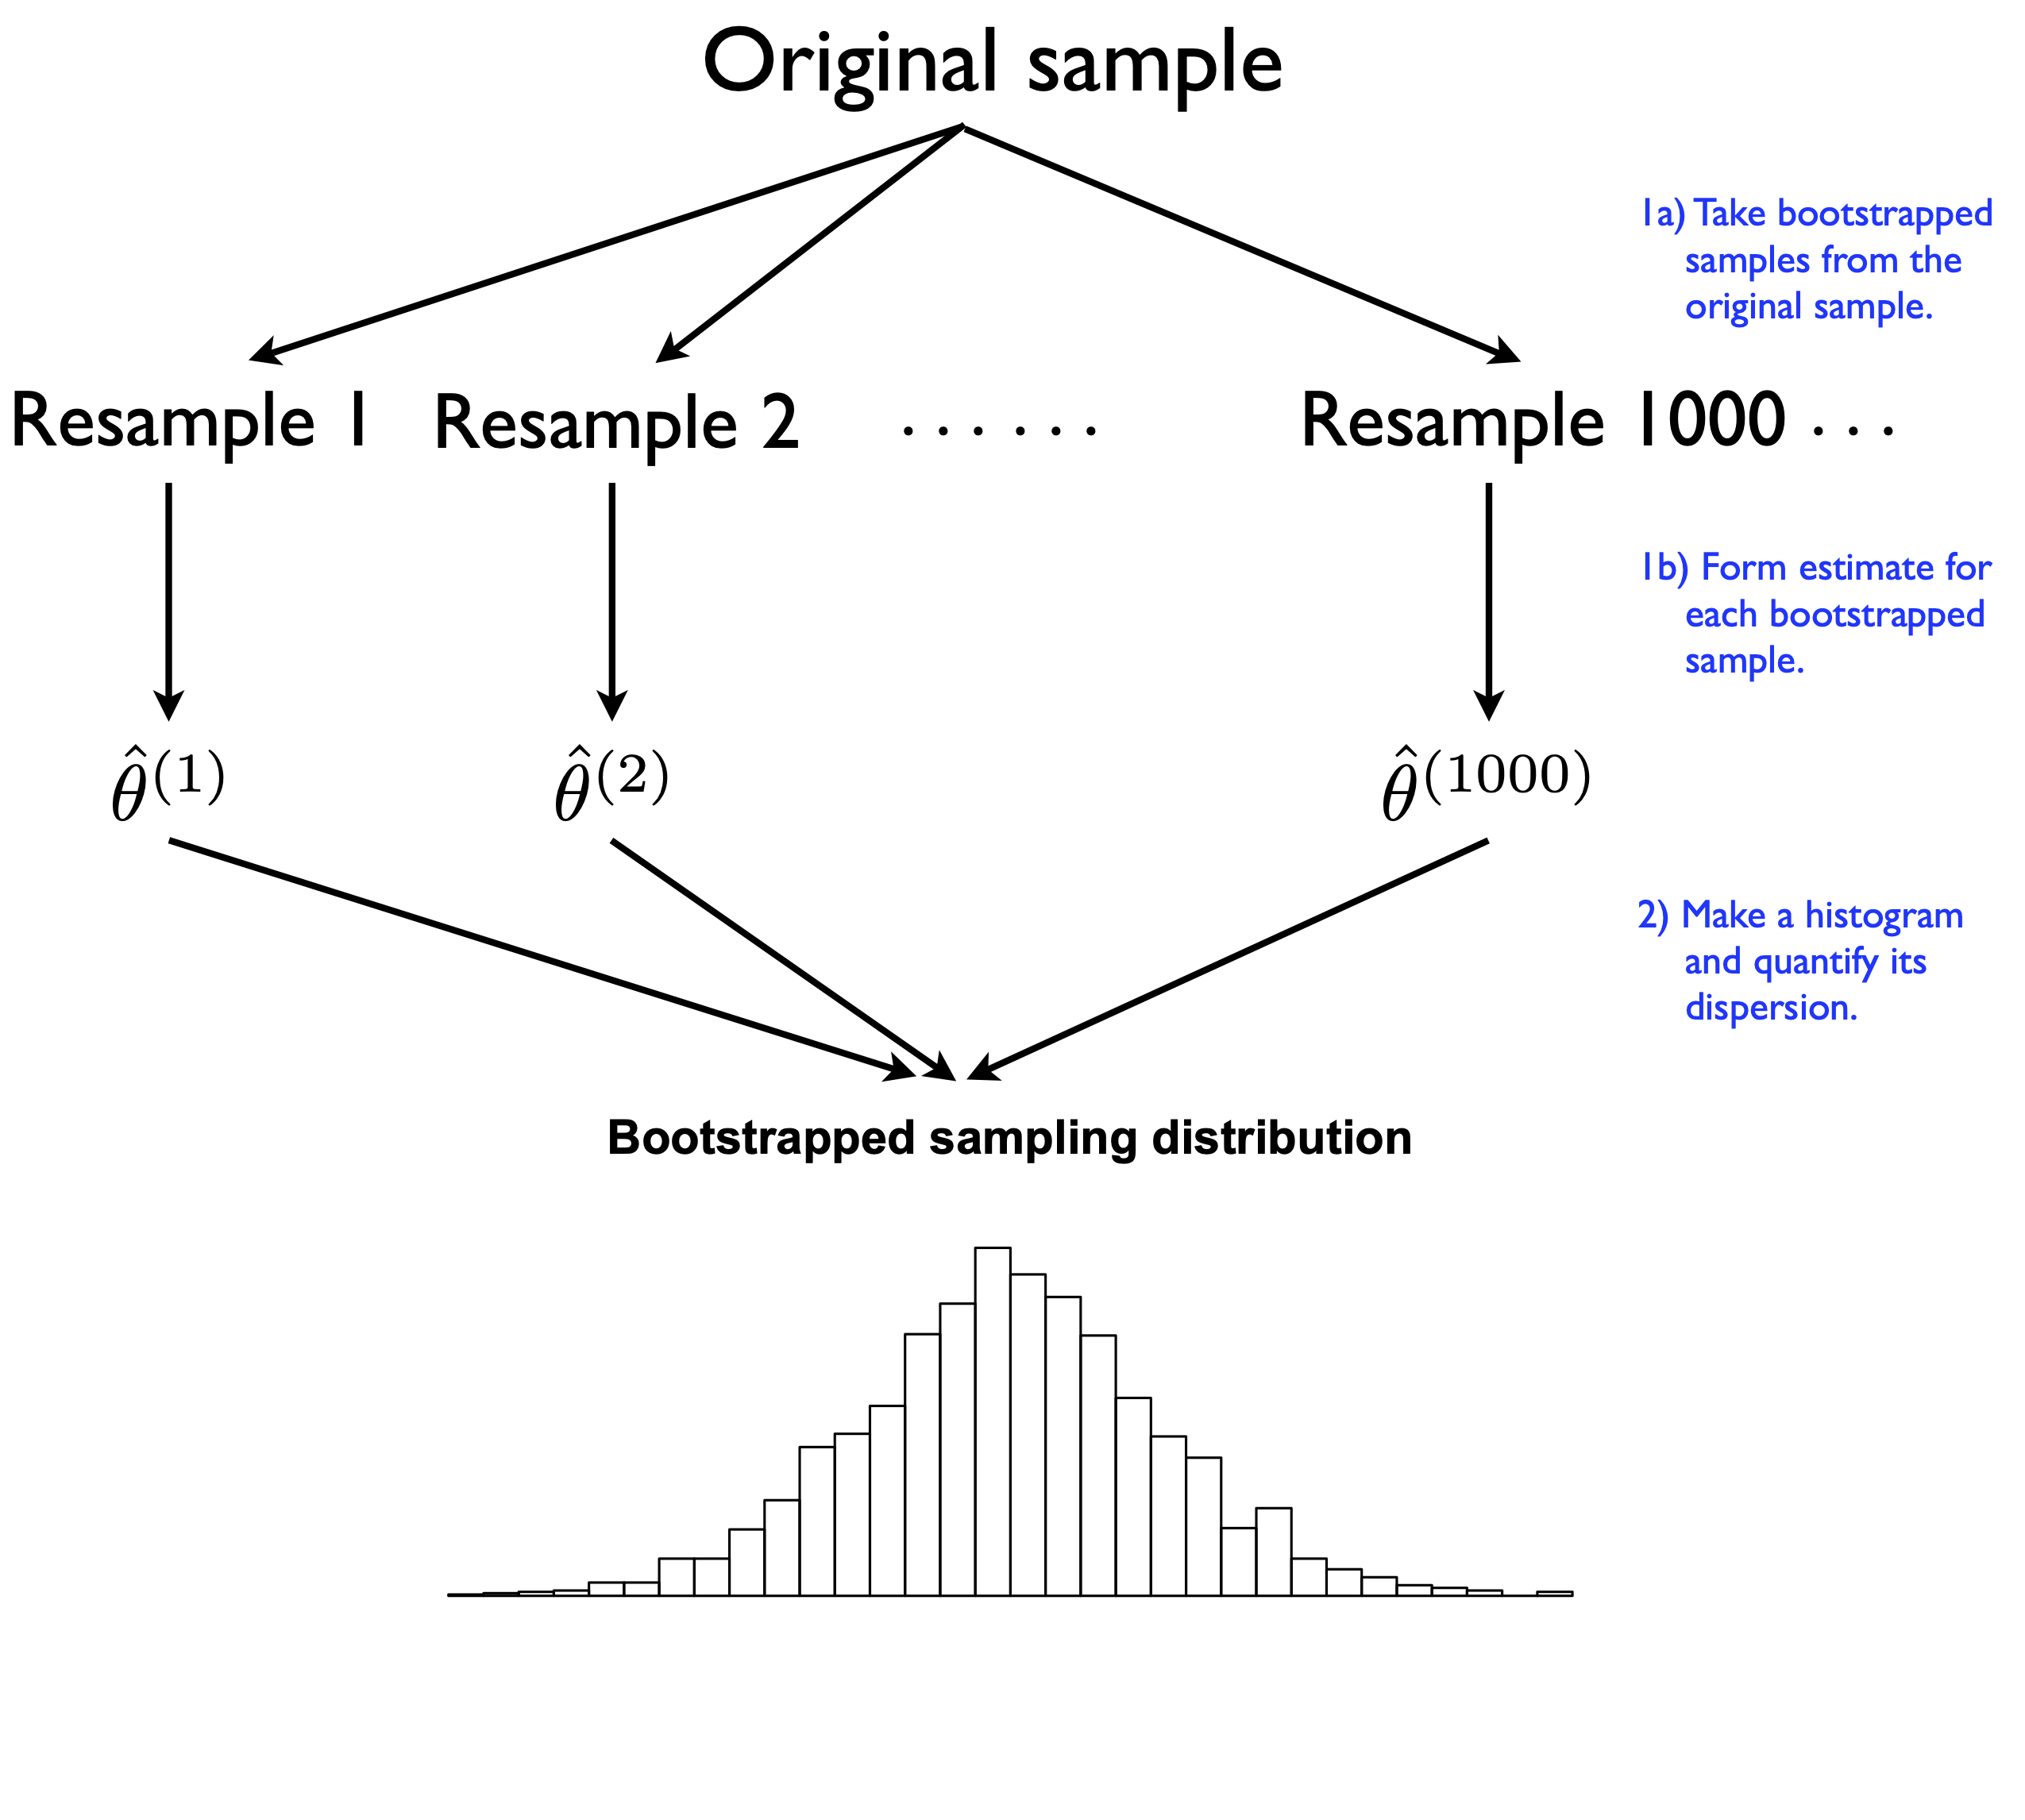
\includegraphics[scale=.4]{figures/bootstrapping_schematic.png}
\end{figure}




% The bootstrap is a important general technique which has sparked in-
% tense interest from both applied and theoretically inclined researchers since
% Efron’s groundbreaking (1979) paper. There are at least a dozen recent
% monographs on the subject among which I would recommend Efron and
% Tibshirani (1993), Davison and Hinkley (1997). At an elementary level the
% paper of Efron and Gong (1983) is still useful, I believe. It contains among
% other things a nice discussion of how to use the bootstrap to evaluate the
% fishing effect discussed in the last lecture. I’ll describe a standard variant
% below, the ”xy” bootstrap that mimics the well known Eicker-White covari-
% ance matrix estimator, and conclude with a brief discussion of the recently
% introduced bag of little bootstraps. There are many other flavors of the
% bootstrap, some of which I will try to mention in class.
% Efron’s bootstrap provides a very general approach to resampling which
% avoids some problems inherent in the systematic resampling of the jackknife.
% In German the expression an den eigenen Haaren aus dem Sumpf zu ziehen
% nicely captures the idea of the bootstrap – “to pull yourself out of the swamp
% by your own hair.” The sample itself is used to assess the precision of the
% estimate ˆθ.
% I will conclude with a prototypical example of the use of the bootstrap.
% An enormous variety of other examples may be found in the books by Efron
% and Tibshirani (1993) and Davison and Hinkley (1997).
% In regression we need not use the residual bootstrap on page 2. A more
% direct implementation of the bootstrap would be to “resample (x, y)-pairs”

 \end{frame}
%----------------------------------------------------------------------%
\subsection{Example: Elasticity of Demand for Gasoline}
%----------------------------------------------------------------------%
%----------------------------------------------------------------------%
\begin{frame}[fragile]
\frametitle{Example: Elasticity of Demand for Gasoline}
\begin{figure}[H] \centering
  \centering
  
\includegraphics[scale=0.35]{figures/baticomputer_meme.jpg}
  \\
  \tiny photo from \url{https://www.dailydot.com/parsec/batman-1966-labels-tumblr-twitter-vine/}
\end{figure}

 \end{frame}
 %----------------------------------------------------------------------%

%----------------------------------------------------------------------%
\begin{frame}[fragile]
\frametitle{Review and Caveats}

\begin{itemize}
  \item The bootstrap is a widely applicable and extremely powerful statistical tool that can be used to quantify the uncertainty associated with a given estimator or statistical learning method. 
  \medskip
  \item The power of the bootstrap, and resampling in general, lies in the fact that it can be easily applied to a wide range of statistical learning methods.
  \medskip
  \item In particular, it does not assume that the regression errors are iid so it can accommodate heteroscedasticity.
 \medskip
  \item Of course it does still assume that the observations are independent. 
  \medskip
  \item Resampling dependent observations is an inherently more difficult task which has generated its own rather large literature. 
\end{itemize}


\end{frame}

%----------------------------------------------------------------------%
%----------------------------------------------------------------------%
\end{document}
